\documentclass{article}
\usepackage{ctex}
\usepackage{listings}
\lstset{tabsize=1}
\usepackage[top=1.5cm]{geometry}
\usepackage{graphicx}
\graphicspath{{picture/}}
\title{git 使用总结}
\author{W.J.Z}
\date{2019.4.9}

\begin{document}
	\maketitle
	\section{git安装与配置}
	\subsection{安装}
	\begin{enumerate}
		\item 发行版基础安装包安装 sudo yum install git
		
		\item 二进制文件安装:	sudo yum install curl-devel expat-devel gettext-devel openssl-devel zlib-devel
		sudo yum install asciidoc xmlto docbook2x \\	
		下载地址:https://github.com/git/git/releases\\	
		tar -zxf git-2.0.0.tar.gz\\
		cd git-2.0.0\\
		make configure\\
		./configure --prefix=/usr\\
		make all doc info\\
		sudo make install install-doc install-html install-info
	\end{enumerate}


	\subsection{配置}
	\begin{enumerate}
		\item /etc/gitconfig 文件: 包含系统上每一个用户及他们仓库的通用配置。 如果使用带有 --system 选项的
		git config 时,它会从此文件读写配置变量
		
		\item ~/.gitconfig 或 ~/.config/git/config 文件:只针对当前用户。 可以传递 --global 选项让 Git
		读写此文件
		
		\item 当前使用仓库的 Git 目录中的 config 文件(就是 .git/config):针对该仓库
		
		\item 用户信息:
		$ git config --global user.name "John Doe"
		$ git config --global user.email johndoe@example.com
		\item 文本编辑器:
		git config --global core.editor emacs
		\item 检查配置信息:
		git config --list
		\item 获取帮助:
		git help config
		
		\item 忽略文件 
		cat .gitignore
	\end{enumerate}


	\section{简单命令}
	\begin{enumerate}
		\item 在现有目录中初始化仓库: git init
		
		\item 跟踪文件:git add *.c
		
		\item 提交文件: git commit -m 'message'
		
		\item 克隆现有仓库:git clone https://github.com/libgit2/libgit2
		
		\item 检查当前文件状态:git status
		
		\item 比较工作目录文件和暂存区文件快照的差异:git diff
		
		\item 比较已经暂存和上次提交之间的差异:git diff -cached
		
		\item 跳过使用暂停区域:git commit -a -m ''
		
		\item 从工作目录中删除文件:git rm\\
		如果已经放入暂存区,则使用git rm -f强制删除
		
		\item 从暂存区和仓库中删除:git rm --cached
		
		\item 移动文件:git mv
		
		\item 查看提交历史:git log
		
		\item 撤销操作:git commit --amend
		
		\item 取消暂存的文件:git reset  HEAD
		
		\item 插销对文件的修改:git checkout --
		
		\item 创建标签:git tag  -a v1.4 -m 'version 1.4'
		
		\item 查看标签对应的提交信息:git show v1.4
		
		\item git别名:git confit --global alias.ci commint
	\end{enumerate} 
	\section{分支}
	\begin{enumerate}
		\item 分支创建:git branch testing
		
		\item  分支切换:git checkout testing
		
		\item 创建分支并转移:git checkout -b testing
		
		\item 删除分支:git branch -d testing
		
		\item 分支合并:git merge testing
		
		\item 分支管理:git branch
		
		
	\end{enumerate}
	\section{gitHub开源项目贡献演示}
	\begin{enumerate}
		\item 将派生的副本复制到本地:https://github.com/sealgull/hellorworld.git
		
		\item 切换到项目文件夹下:cd helloworld/
		
		\item 创建分支:git checkout -b author
		
		\item 进行修改提交仓库:git commit -a -m ''
		
		\item 推送到远程服务器:git push origin author 输入用户名和密码即可
		
		\item 进行比较并推送:compare \& pull request
		
		\item 创建后项目原有者就会收到合并请求,之后进行交流。
		
		\item permission denied 解决方法
		
	\end{enumerate}
	\begin{figure}[h]
		\centering
		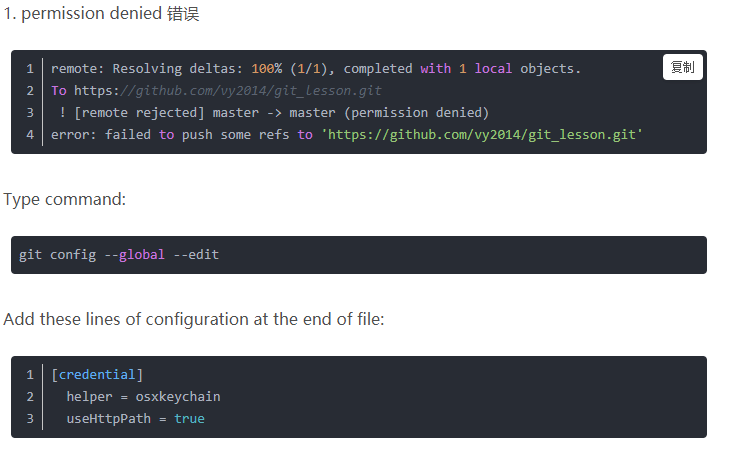
\includegraphics[scale=0.5]{1}
	\end{figure}

	\section{同步开源项目别人的更新}
	\begin{enumerate}
		\item git remote -v 查看远程主机
		\item git remote add upstream git@github.com:xxx/xxx.git 添加远程主机
		\item git fetch upstream 从源库更新代码
		\item git merge upstream/master 合并到本地代码
		\item git push 同步自己的远程代码
		\item git remote remove upstream 删除远程主机
	\end{enumerate}
\end{document}